\documentclass[10pt]{article}
\usepackage[spanish]{babel}
\usepackage{graphicx}
\usepackage{tabularx} % para width table
\usepackage[left=1.5cm,top=2.4cm,right=2.1cm,bottom=3cm,bindingoffset=0.5cm]{geometry} % original[22 iz,24 arri]
\usepackage{multirow}
\graphicspath{{img/}{img1/}}
\usepackage{url}
\usepackage{amsmath}
\usepackage{hyperref} % Hipervinculos
\usepackage{ragged2e} % Alineación
\usepackage{amssymb} %therefore
\usepackage{float} %Here
\usepackage{listings}



%% pregunta 2
\usepackage{url}
\usepackage{comment}
\usepackage{mathrsfs}
\newsavebox\foobox
\newlength{\foodim}
\newcommand{\slantbox}[2][0]{\mbox{%
		\sbox{\foobox}{#2}%
		\foodim=#1\wd\foobox
		\hskip \wd\foobox
		\hskip -0.5\foodim
		\pdfsave
		\pdfsetmatrix{1 0 #1 1}%
		\llap{\usebox{\foobox}}%
		\pdfrestore
		\hskip 0.5\foodim
}}
\def\Laplace{\slantbox[-.45]{$\mathscr{L}$}}

\setlength{\parindent}{25pt}


\usepackage{pdfpages} %Incluir pdf
\begin{document}
	
	\newcommand{\iu}{{i\mkern1mu}}
	\addtolength{\jot}{1em}

	
	\centering
	\begin{tabular}{ |	p{30 mm}|	p{61 mm}	|	p{33mm}	| p{43mm}	| } 
		\hline
		
		
		\multirow{4}{30mm}{\centering 
\includegraphics[scale=0.22]{logo}} &
		\multirow{4}{61mm}{\centering \textbf{ \textbf{Manual de prácticas del Laboratorio de Análisis de Sistemas y Señales}}}    & Código: & MADO-76 \\
		\cline{3-4}
		& &  Versión & 01 \\
		\cline{3-4}
		& & Página: & 40/97 \\ \cline{3-4}
		& & Sección ISO: & 8.3 \\ \cline{3-4}
		& & Fecha de emisión: & 28 de frebrero 2019 \\
		\hline
	\end{tabular}
\begin{tabular}{ |	c |	c	| } 
	
	\multirow{2}{65mm}{ \centering Facultad de ingeniería} &
	\multirow{2}{111mm}{\centering \textbf{ Area/Departamento: \\ Laboratorio de control y robótica}}   \\
	& \\ \hline
\end{tabular}
\begin{tabular}{|p{180mm}|}
	\multirow{1}{180mm}{ \centering La impresion de este documento es una copia no controlada }  \\ \hline \end{tabular} \\

\vspace{1cm}

{\centering \Large Práctica N◦3 Transformada Z y aplicaciones a sistemas de tiempo discreto }

\hspace{5cm}

\begin{figure}[!h]
	\centering
	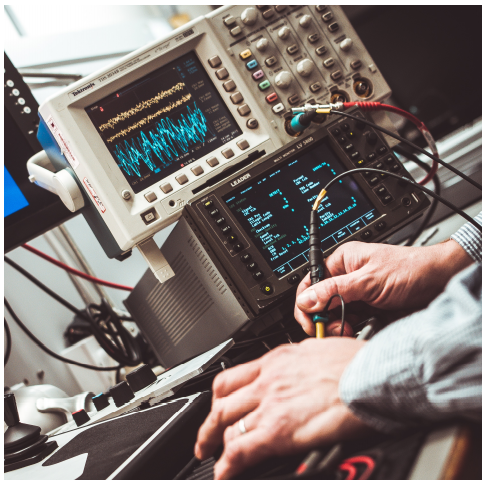
\includegraphics[scale=0.7]{portada.png}
\end{figure}

\hspace{1cm}
\begin{tabular}{|c| p{122mm}|}
	\hline
	\multirow{4}{50mm}{\\ \centering \large Apellidos y nombres}	 &  \\  
	& Alfaro Domínguez Rodrigo  \\  \cline{2-2}
	&  \\  
	& Barrera Peña Víctor Miguel \\  \cline{2-2}
	&  \\  
	& Villeda Hernández Erick Ricardo \\ 
	\hline
\end{tabular}
\begin{tabular}{|p{50mm} | c | p{80mm}| p{23mm} |}
	Grpo: & 4 & \multirow{2}{90mm}{Profesor: M.I Lauro Fernando Vazquez Alberto } & Calificación \\ \cline{1-2}
	Brigada: & 1 &  &\\ \hline
	Semestre: & 2021-1 & Fecha de ejecución: 22/09/2020-- 29/09/2020 & \\ \hline
\end{tabular}





	\includepdf[pages={2-11}]{latex/practica2.pdf}
%	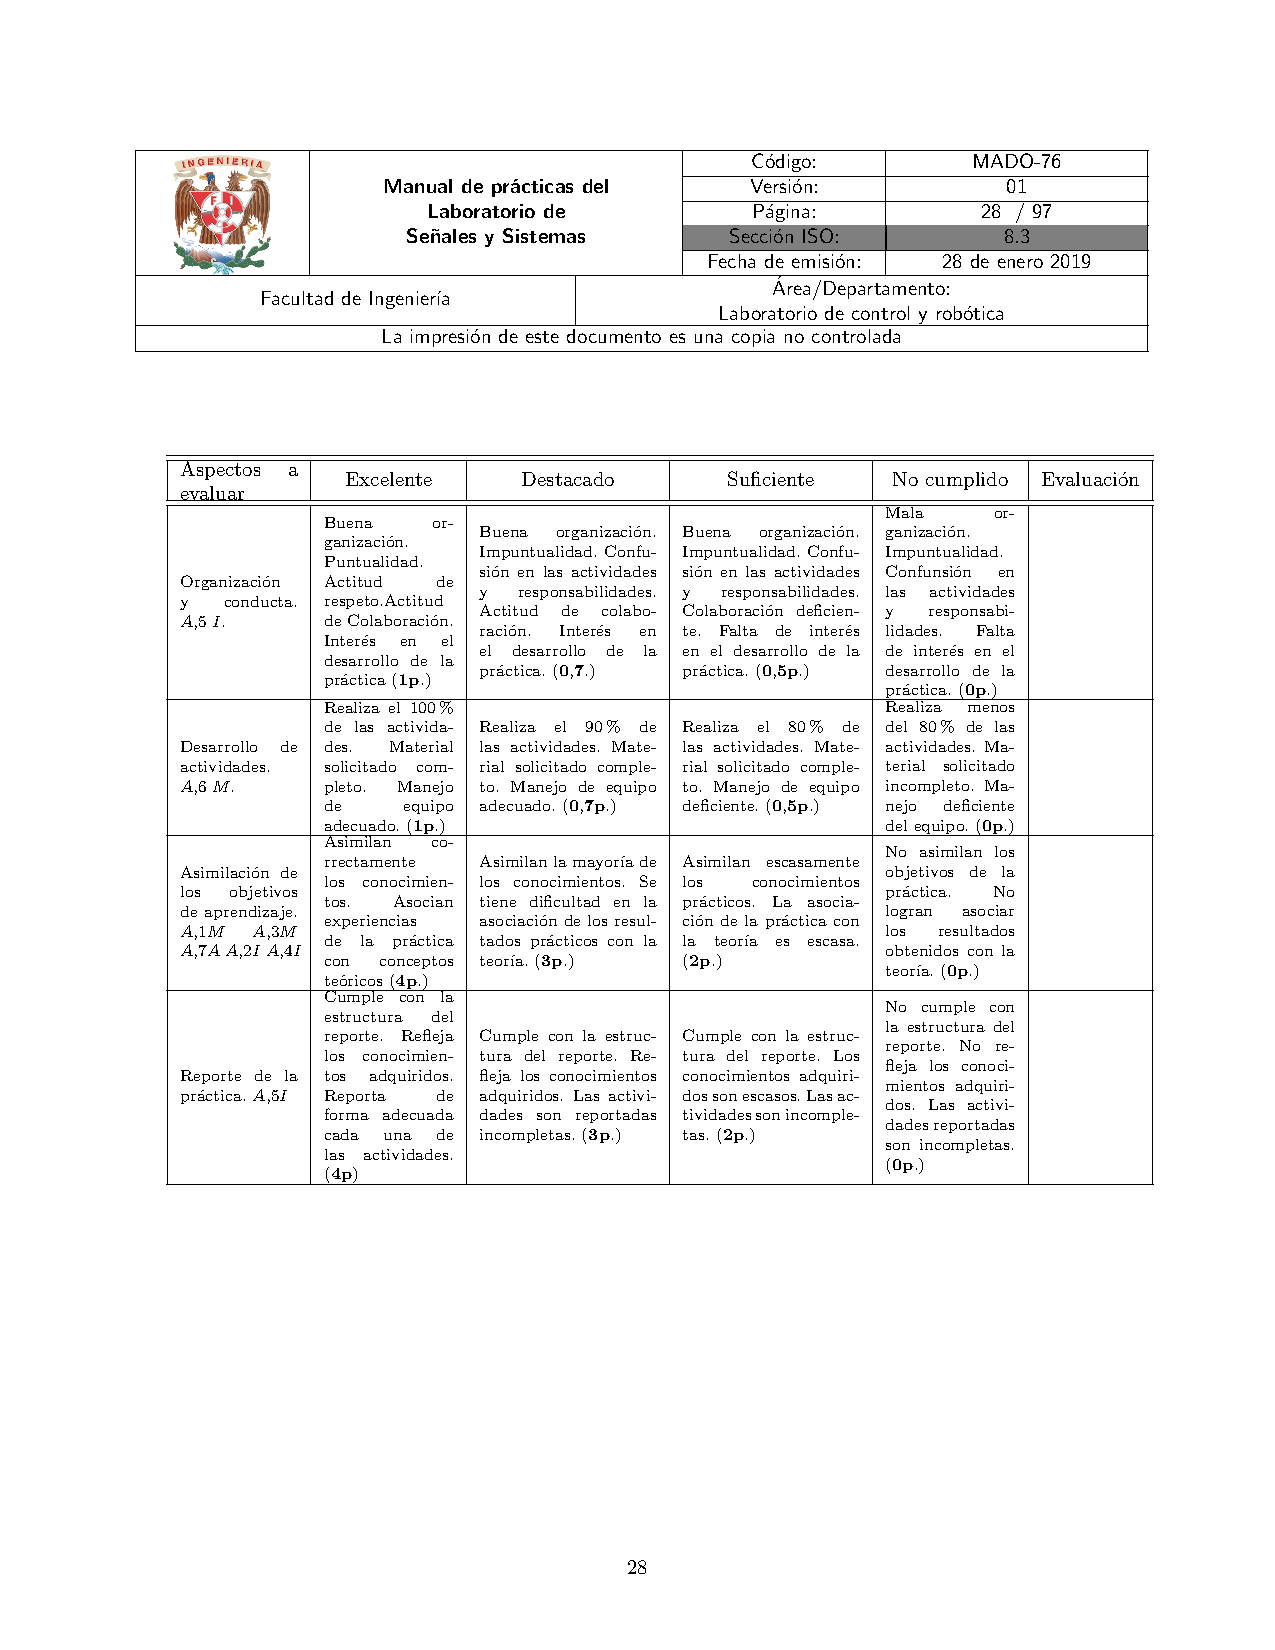
\includepdf[pages=-]{latex/parte1.pdf}
%	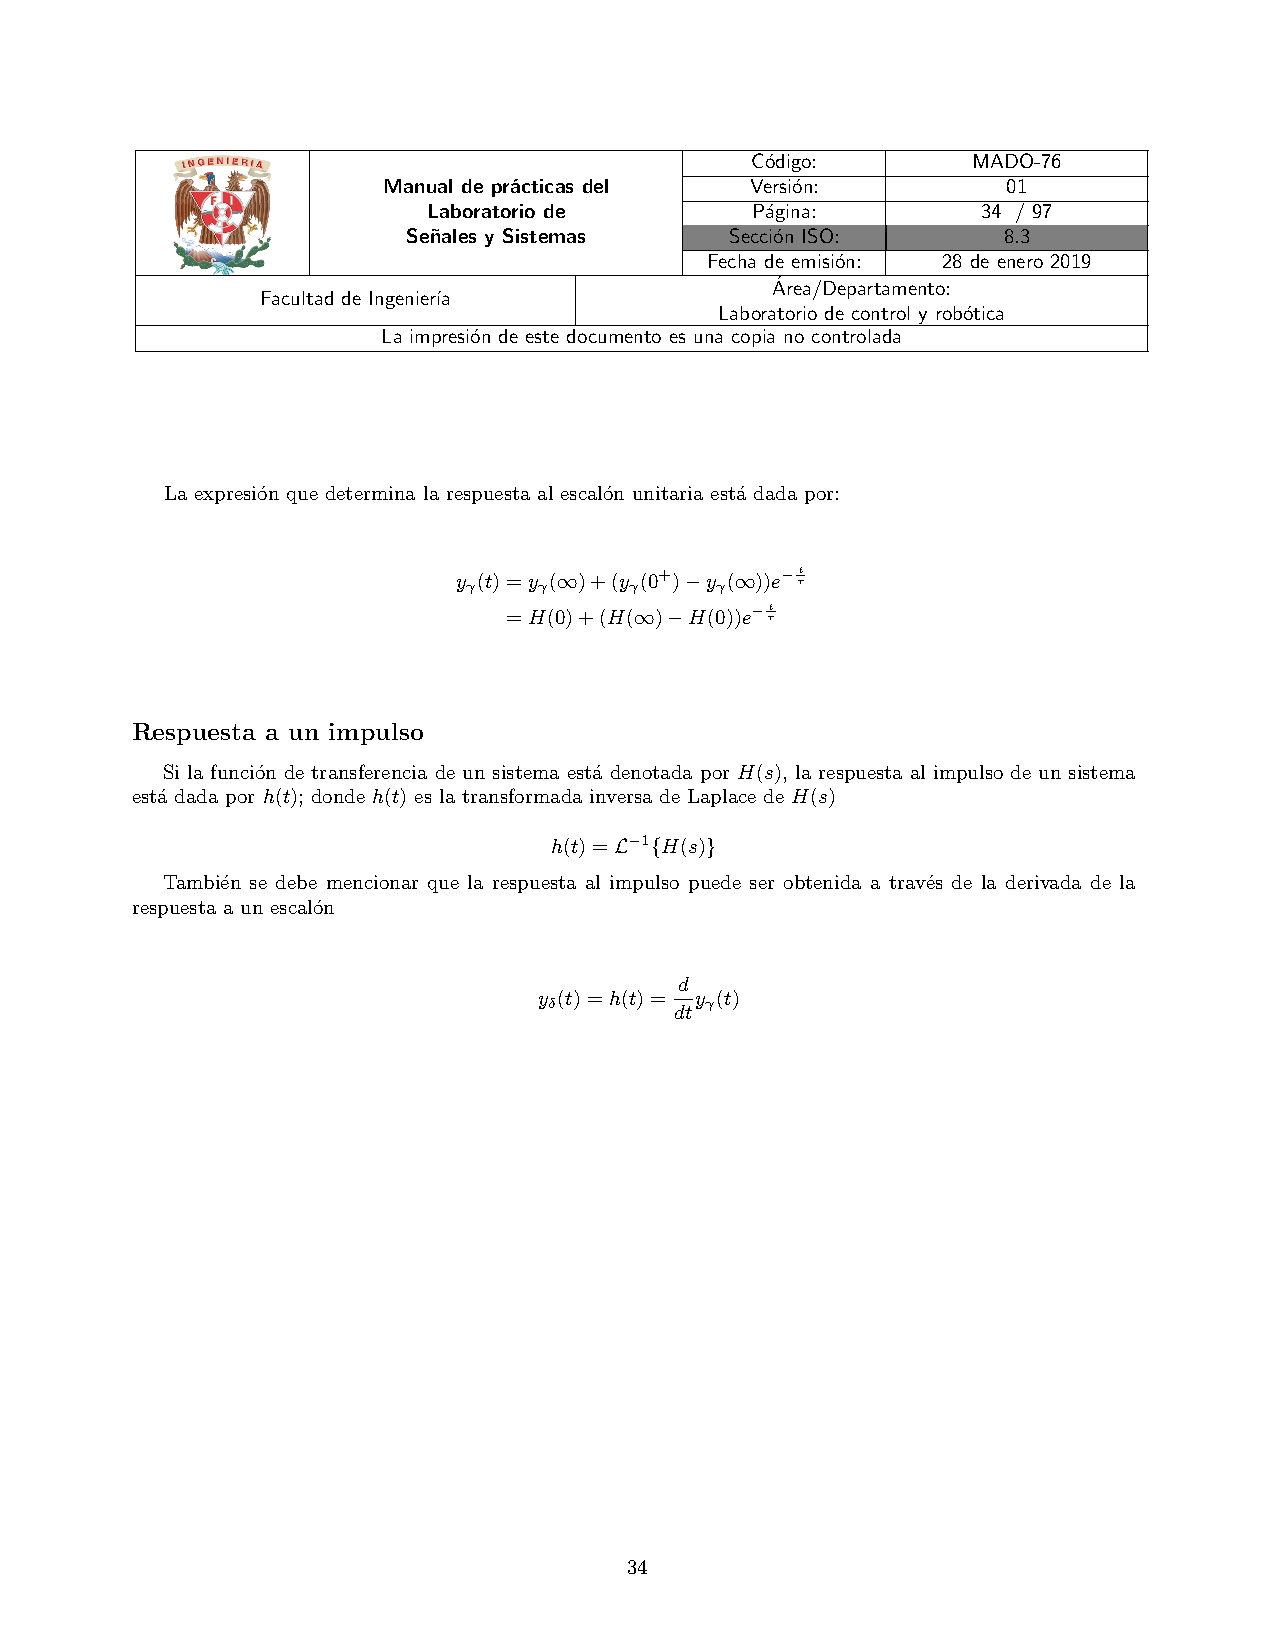
\includepdf[pages=-]{latex/parte2.pdf}
%	\noindent \justifying

\section{Previo}

\subsection{Identificar un sistema dinámico que se tenga en casa y definir la salida y la entrada del mismo (para discusión en clase)}
\subsection{¿Como analizaría un sistema de orden mayor?}
Para analizar un sistema de orden superior empezamos por escribir su función de transferencia:
\begin{equation}
H(s)=K\frac{(s-z_1)(s-z_2)...(s-z_n)}{(s-p_1)(s-p_2)(s-p_n)}
\end{equation} 
La mayor parte de la información de como funciona el ssitema nos la darán la localización de los polos y ceros. Esto determina si el sistema es estable o no.\\
En caso de tener polos reales la ecuación toma la siguiente forma:
\begin{equation}
H(s)=\frac{a_1}{s-p_1}+...+\frac{a_n}{s-p_n}
\end{equation}
A partir de aquí analizamos su respuesta a un impulso y un escalón, quedándonos sus ecuaciones de una de las siguientes formas respectivamente:
\begin{equation}
y_{imp}=\alpha_1 e^{p_1t}+..+\alpha_n e^{p_nt}
\end{equation}
\begin{equation}
y_{step}=\beta_0 + \beta_1 e^{p_1t}+...+ \beta_n e^{p_nt}
\end{equation}
Cada polo real p genera un término exponencial en la respuesta. El comportamiento de las osilaciones va a depender de si la parte real del poplo es negativa o positiva, mientras que la magnitud depende de los ceros.\\
En el caso de un sistema de segundo orden podemos escribir su ecuación característica en términos de zeta y omega, de la siguiente forma:
\begin{equation}
\frac{d^2y(t)}{dt^2}+2\zeta \omega_n \frac{dy(t)}{dt}+(\omega_n)^2y(t)=k(\omega_n)^2x(t)
\end{equation}
A partir de su respuesta en la ecuación homogénea podemos llegar a un polinimio de la siguiente forma:
\begin{equation}
s^2+2\zeta\omega_ns+\omega^2_n=0
\end{equation}
La respuesta del sistema va a depender de los valores que tenga el término $\zeta$, siendo sus valores posibles entre cero e infinito positivo. Lo que nos interesará para el diseño de un sistema es que su valor sea mayor o igual a uno.
\subsection{¿Cuál es la importancia de la constante de tiempo $\tau$ y el factor de amortiguamiento $\zeta$ ?}


%	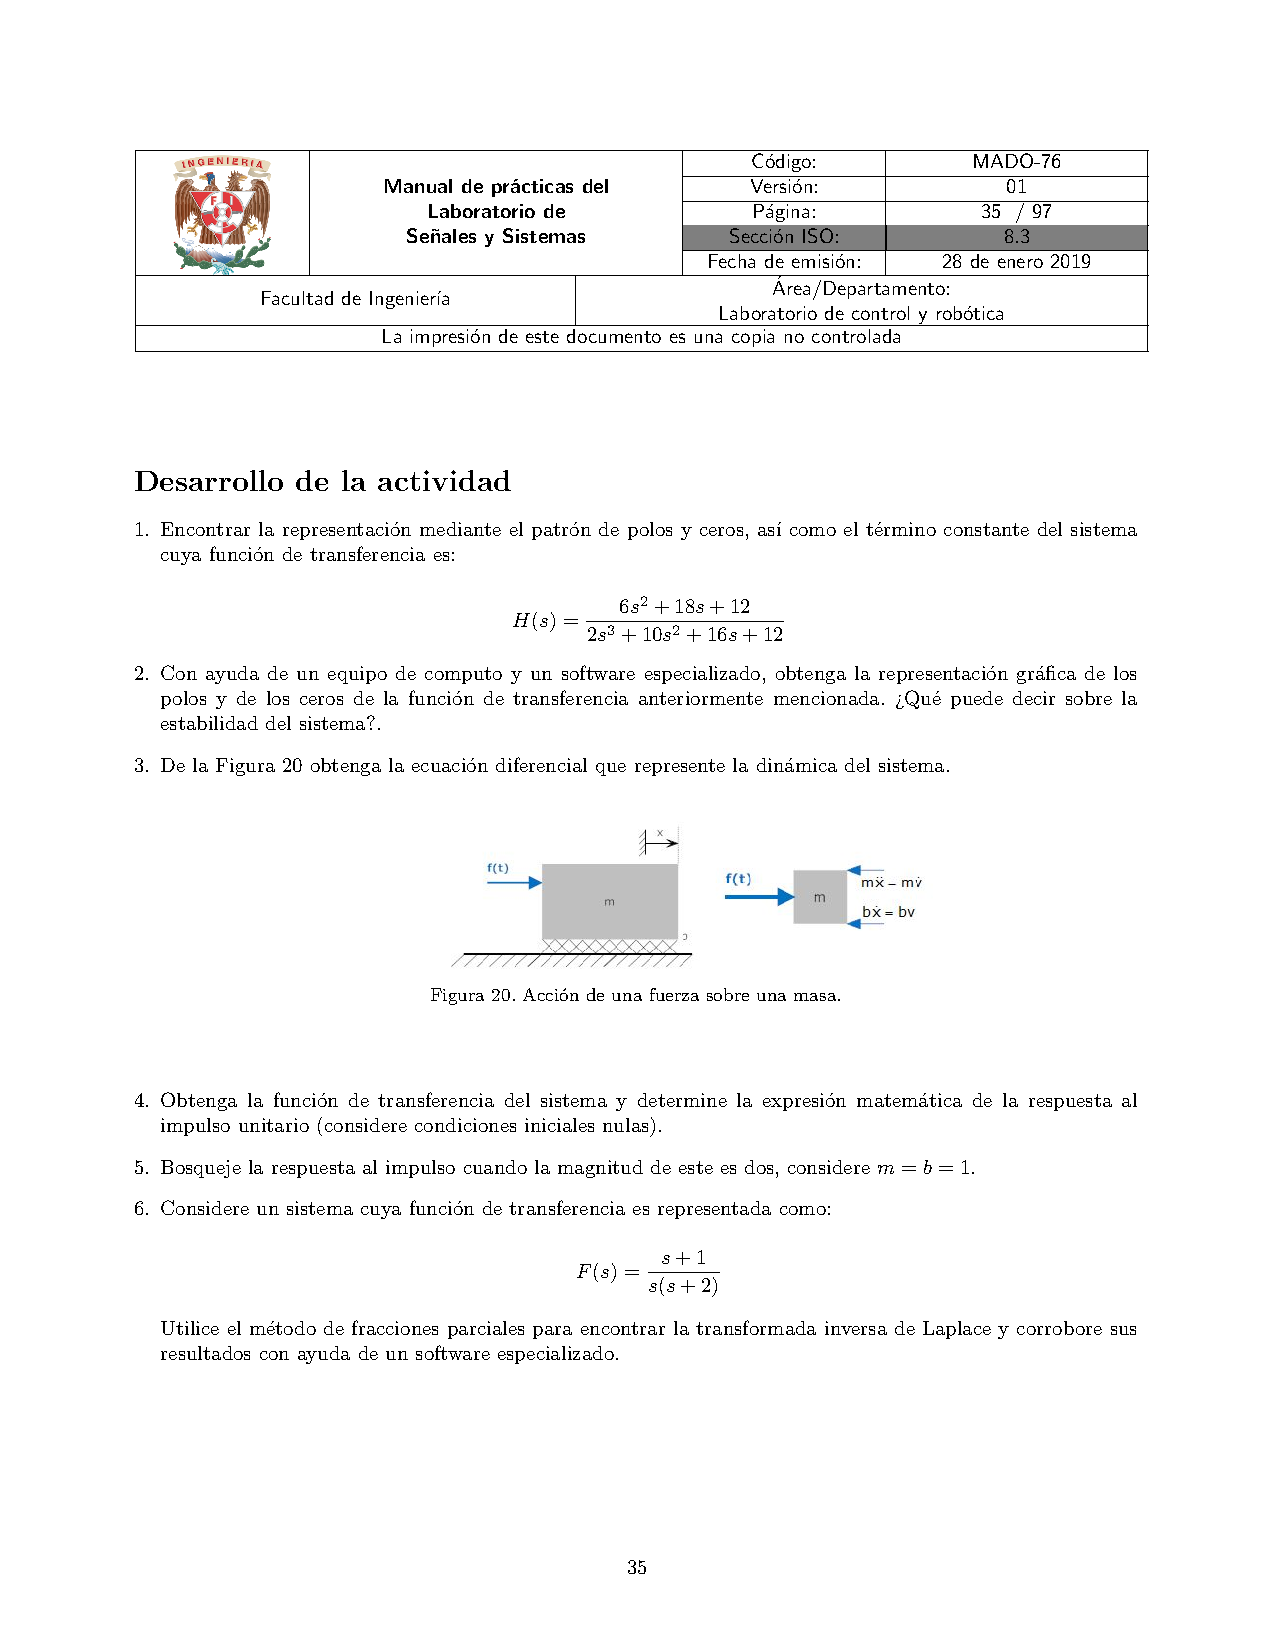
\includepdf[pages=-]{latex/parte3.pdf}
	
	\section{Solución desarrollo}
\subsection{Actividad 1}

\noindent\textbf{1. Encontrar la representación mediante el patrón de polos y ceros, así como el término constante del sistema cuya función de transferencia es:}
	\begin{equation}
		H(s)=\frac{6s^2+18s+12}{2s^3+10s^2+16s+12}
	\end{equation}
	\newline
	
	Término constante
	\begin{equation}
		H(s)=\frac{6s^2+18s+12}{2s^3+10s^2+16s+12}
	\end{equation}
	\begin{equation}
		\Rightarrow H(s)=\frac{6*\frac{6s^2}{6}+\frac{18s}{6}+\frac{12}{6}}{2*\frac{2s^3}{2}+\frac{10s^2}{2}+\frac{16s}{2}+\frac{12}{2}}
	\end{equation}
	\begin{equation}
		\Rightarrow H(s)=\frac{6*(s^2+3s+2)}{2*(s^3+5s^2+8s+6)}
	\end{equation}
	\begin{equation}
		\Rightarrow H(s)=3*\frac{s^2+3s+2}{s^3+5s^2+8s+6}
	\end{equation}	
	\begin{equation}
		\Rightarrow Termino Constante = 3
	\end{equation}
	
	Raíces
	\begin{equation}
		H(s)=\frac{s^2+3s+2}{s^3+5s^2+8s+6}
	\end{equation}	
	\begin{equation}
		\Rightarrow H(s)=\frac{(s+2)(s+1)}{(s+3)(s^2+2s+2)}
	\end{equation}		
	\begin{equation}
		\Rightarrow c_1=-2,c_2=-1,c_3=-3,c_4=1+\iu,c_5=1-\iu
	\end{equation}		
	
	\noindent Debido a que los polos son las raíces del denominador y los ceros las raíces del numerador llegamos a que
	\begin{equation}
		Ceros: c_1=-2,c_2=-1 
	\end{equation}		
	\begin{equation}
		Polos: c_3=-3,c_4=1+\iu,c_5=1-\iu
	\end{equation}
	\newline
	
\subsection{Actividad 2}

\subsection{Actividad 3}
\noindent\textbf{3. De la Figura 20 obtenga la ecuación diferencial que represente la dinámica del sistema.}	
\[
f(t)=x(t){\Longrightarrow}Entrada.
\]
\[
x=y(t){\Longrightarrow}Salida.
\]
\[
m:masa.
\]
\[
b:fricción.
\]
\[
f(t)-m{\"x}-b{\.x}=0
\]
\[
f(t)=m{\"x}+b{\.x}
\]
\[
\therefore x(t)=m{\"y}+b{\.y}
\]


\subsection{Actividad 4}
	
	\noindent\textbf{4.  Obtenga la función de transferencia del sistema y determine la expresión matemática de la respuesta impulso unitario (considere condiciones iniciales nulas):
	\begin{equation}
		S=\frac{1}{ms^2+bs}=\frac{1}{s(ms+b)=\frac{A}{s}+\frac{B}{ms+b}}
	\end{equation}
	\begin{equation}
		\Rightarrow 1=A(ms+b)+Bs
	\end{equation}
	Si s = 0
	\begin{equation}
		\Rightarrow 1=A(m*0+b)+B*0
	\end{equation}
	\begin{equation}
		\Rightarrow 1=A(b)
	\end{equation}
	\begin{equation}
		\Rightarrow A=\frac{1}{b}
	\end{equation}
	Si s=$\frac{-b}{m}$
	\begin{equation}
		\Rightarrow 1=A(m*\frac{-b}{m}+b)+B(\frac{-b}{m})
	\end{equation}
	\begin{equation}
		\Rightarrow 1=A(-b+b)+B(\frac{-b}{m})
	\end{equation}
	\begin{equation}
		\Rightarrow 1=A(0)+B(\frac{-b}{m})
	\end{equation}
	\begin{equation}
		\Rightarrow 1=B(\frac{-b}{m})
	\end{equation}
	\begin{equation}
		\Rightarrow B=\frac{m}{-b}
	\end{equation}
	Por lo tanto, tras sustituir A y B obtenemos
	\begin{equation}
		S=\frac{1}{s(b)}-\frac{-m}{b(ms+b)}=\frac{1}{b}\frac{1}{s}-\frac{m}{mb}\frac{1}{s+\frac{b}{m}}
	\end{equation}
	Si aplicamos función de Laplace inversa a este resultado obtenemos
	\begin{equation}
		y(t)=\frac{1}{b}u(t)-\frac{1}{b}e^{-\frac{b}{m}*t}
	\end{equation}
	\newline
	
\subsection{Actividad 5}

\subsection{Actividad 6}
\noindent\textbf{6. Considere un sistema cuya función de transferencia es representada como:
\[
F(s)=\frac{s+1}{s(s+2)}
\]
Utilice el método de fracciones parciales para encontrar la transformada inversa de Laplace y corrobore sus resultados con ayuda de un software especializado.}	
\[
\frac{s+1}{s(s+2)}=\frac{A}{s}+\frac{B}{s+2}{\Longrightarrow}(1)
\]
Multiplicamos la expresión (1) por s(s+2).
\[
(\frac{s+1}{s(s+2)})*s(s+2)=(\frac{A}{s}+\frac{B}{s+2})*s(s+2)
\]
\[
s+1=A*(s+2)+B*(s){\Longrightarrow}(2)
\]
Para poder encontar los valores de A y B primeramente vamos a sustituir de la expresión (2) los valores de s por 0, y vamos a resolver.
\[
\textbf{s=0:}
\]
\[
s+1=A*(s+2)+B*(s)
\]
\[
0+1=A*(0+2)+B*(0)
\]
\[
1=A*2
\]
\[
\frac{1}{2}=A
\]
\[
\therefore A=\frac{1}{2}
\]
Para poder encontrar el valor de B, vamos a sustituir el valor de s, igualmente de la expresión (2) por -1, y vamos a resolver.
\[
\textbf{s=-1:}
\]
\[
s+1=A*(s+2)+B*(s)
\]
\[
-1+1=A*(-1+2)+B*(-1)
\]
\[
0=A*(1)-B
\]
\[
0=A-B
\]
\[
A=B
\]
\[
\therefore B=\frac{1}{2}
\]
Sustituimos los valores de A y B en la expresión (1).
\[
\frac{s+1}{s(s+2)}=\frac{\frac{1}{2}}{s}+\frac{\frac{1}{2}}{s+2}
\]
\[
F(s)=\frac{1}{2}\frac{1}{s}+\frac{1}{2}\frac{1}{s+2}
\]
\[
\mathcal{L}^{-1}=\mathcal{L}^{-1}
\]
\[
\therefore{y(t)=\frac{1}{2}\mathscr{U}(t)+\frac{1}{2}e^{-2t}}
\]
Comprobación en MATLAB:
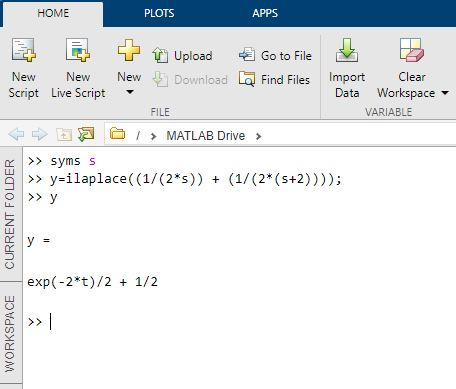
\includegraphics[scale=0.8, angle=0]{mAT.JPG}

\subsection{Actividad 7}
\subsection{Actividad 8}

\subsection{Actividad 9}
\noindent\textbf{9. De una forma alternativa, considerando el teorema del valor final y el teorema del valor inicial (sin la transformada inversa de Laplace) determine la respuesta al escalón. ¿Qué puede decir con respecto a lo realizado en la actividad 8?.}
\[
y(s)=\frac{3s+1}{s(5s+1)}
\]
\[
\lim_{s \to \infty}y(s)=\lim_{s \to \infty}\frac{3s+1}{s(5s+1)}
\]
\[
\lim_{s \to 0}y(s)=\lim_{s \to 0}\frac{3s+1}{s(5s+1)}
\]
Para poder utilizar el teorema del valor inicial y del valor final, debemos hacer que nuestra expresión tenga la siguiente estructura:
\[
H(s)=\frac{1}{s}\frac{bs+c}{(s+a)}
\]
Para ello vamos a dividir tanto el numerador como denominador entre 5, y vamos a reacomodar.
\[
=\frac{\frac{1}{5}}{\frac{1}{5}}\frac{3s+1}{s(5s+1)}
\]
\[
=\frac{\frac{3s+1}{5}}{s{\frac{5s+1}{5}}}
\]
\[
=\frac{1}{s}\frac{\frac{3}{5}s+\frac{1}{5}}{s+\frac{1}{5}}
\]
\[
a=\frac{1}{5};b=\frac{3}{5};c=\frac{1}{5}
\]
Una vez que tenemos nuestra  expresión con la estructura de H(s), vamos a ver que por definición tenemos lo siguiente:
\[
H(\infty)=b
\]
\[
H(0)=\frac{c}{a}
\]
Por lo tanto:
\[
\lim_{s \to \infty}y(s)=H(\infty)=b=\frac{3}{5}=0.6
\]
\[
\lim_{s \to 0}y(s)=H(0)=\frac{c}{a}=\frac{\frac{1}{5}}{\frac{1}{5}}=
\frac{5*1}{5*1}=1
\]
A través del teorema del valor inicial y el valor final, podemos llegar a los mismos valores (inicial y final), y esto se puede comprobar con la grafica obtenida en el inciso 8), ya que muestra los mismos valores.

	\section{Observaciones y conclusiones}

\begin{itemize}
	\item \textbf{Alfaro Domínguez Rodrigo:}
	\item \textbf{Barrera Peña Víctor Miguel:} 
	\item \textbf{Villeda Hernández Erick Ricardo:}
	
\end{itemize}
	
	
	\subsection*{Referencias}
	
	\begin{itemize}
		\item Aström K., Murray R., (2004), Analysis and Design of Feedback Systems, Preprint, University of California.
		\item Baraniuk, R.(19 de diciembre de 2013).\textit{ Polos y Ceros}. Cnx. Recuperado el 2 de octubre  de 2020 de
		\subitem https://cnx.org/contents/ydI5iGfF@2/Polos-y-Ceros	
		\item Mata G., Sánchez V., Gómez J., (2017), Análisis de sistemas y señales con cómputo avanzado, México D.F., Universidad Nacional Autónoma de México.
		\item Maria Alicia Piñeiro. (2020, 10 abril). Transformada de Laplace (parte 1). YouTube. 
		\subitem https://www.youtube.com/watch?v=i1wRqo\_2zgw
		
		\item	S.A. (17 de abril de 2013).\textit{ Unidad III: Transformada de Laplace}. Itpn. Recuperado el 02 de octubre de 2020 de http://itpn.mx/recursosisc/4semestre-/ecuacioneslineales/Unidad-20III.pdf
	\end{itemize}
	
	
\end{document}

